\documentclass[12pt]{article}


\usepackage{amsmath, amssymb, amsfonts}
\usepackage{tikz}
\usepackage{listings}
\usepackage{xcolor}
\usepackage{graphicx}
\usepackage{hyperref}
\usepackage{bm}
\usepackage{enumitem}

\hypersetup{
  colorlinks=true,
  linkcolor=blue,
  filecolor=magenta,
  urlcolor=cyan,
  pdftitle={Data Analysis Script},
  bookmarks=true
}

% Title page customization
\title{Ashutosh Kumar Jha}
\author{12340390}
\date{\today}  % Automatically inserts today's date

\lstset{
    language=Python,
    basicstyle=\ttfamily\small,
    keywordstyle=\color{blue},
    commentstyle=\color{green},
    stringstyle=\color{red},
    showstringspaces=false,
    numbers=left,
    numberstyle=\tiny\color{gray},
    breaklines=true,
    frame=single,
}

\begin{document}

% Create the title page
\maketitle
\thispagestyle{empty}  % Removes page number on the title page

\subsection*{Solution 1}

To solve this problem, we analyze the first digit \( x \) when sampling uniformly from the numbers 1 to 1000.

\subsubsection*{Step 1: Distribution of \( x \)}
The first digit \( x \) can range from 1 to 9. For a uniform distribution from 1 to 1000, the probability \( p_x \) of each digit \( x \) is determined by the proportion of numbers in the range that begin with \( x \). Specifically:
\[
p_x = \frac{\text{Number of integers with first digit } x}{1000}.
\]

#### Case-by-case analysis:
- For \( x = 1 \), the numbers are 1, 10 to 19, 100 to 199:
  \[
  \text{Count} = 1 + 10 + 100 = 111.
  \]
  Therefore, \( p_1 = \frac{111}{1000} = 0.111 \).

- For \( x = 2 \), the numbers are 2, 20 to 29, 200 to 299:
  \[
  \text{Count} = 1 + 10 + 100 = 111.
  \]
  Similarly, \( p_2 = 0.111 \).

- The same logic applies for \( x = 3, 4, \dots, 9 \), as all have the same structure.

Hence, the probabilities are:
\[
p_1 = p_2 = \dots = p_9 = 0.111.
\]

\subsubsection*{Step 2: Verification of Probabilities}
To ensure the probabilities sum to 1:
\[
\sum_{x=1}^9 p_x = 9 \cdot 0.111 = 1.
\]

Thus, the probabilities are correctly normalized.

\subsubsection*{Step 3: Mean of \( x \)}
The mean \( \mu \) of \( x \) is given by:
\[
\mu = \sum_{x=1}^9 x \cdot p_x.
\]
Substituting \( p_x = 0.111 \) for all \( x \):
\[
\mu = \sum_{x=1}^9 x \cdot 0.111 = 0.111 \cdot (1 + 2 + 3 + \dots + 9).
\]
The sum of integers from 1 to 9 is:
\[
1 + 2 + \dots + 9 = \frac{9 \cdot (9 + 1)}{2} = 45.
\]
Therefore:
\[
\mu = 0.111 \cdot 45 = 5.0.
\]

\subsubsection*{Step 4: Variance of \( x \)}
The variance \( \sigma^2 \) of \( x \) is given by:
\[
\sigma^2 = \sum_{x=1}^9 p_x \cdot (x - \mu)^2.
\]
Expanding \( (x - \mu)^2 \):
\[
\sigma^2 = \sum_{x=1}^9 p_x \cdot x^2 - \mu^2.
\]
First, compute \( \sum_{x=1}^9 p_x \cdot x^2 \):
\[
\sum_{x=1}^9 p_x \cdot x^2 = 0.111 \cdot (1^2 + 2^2 + \dots + 9^2).
\]
The sum of squares of integers from 1 to 9 is:
\[
1^2 + 2^2 + \dots + 9^2 = \frac{9 \cdot (9 + 1) \cdot (2 \cdot 9 + 1)}{6} = \frac{9 \cdot 10 \cdot 19}{6} = 285.
\]
Thus:
\[
\sum_{x=1}^9 p_x \cdot x^2 = 0.111 \cdot 285 = 31.635.
\]
Finally, compute the variance:
\[
\sigma^2 = 31.635 - (5.0)^2 = 31.635 - 25.0 = 6.635.
\]

\subsubsection*{Final Results}
The probabilities are:
\[
p_1 = p_2 = \dots = p_9 = 0.111.
\]

The mean and variance of \( x \) are:
\[
\mu = 5.0, \quad \sigma^2 = 6.635.
\]

\subsubsection*{Diagram Representation}
\begin{center}
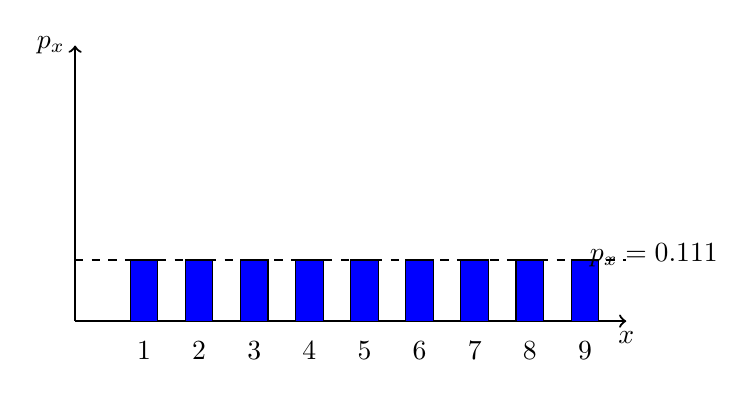
\begin{tikzpicture}[scale=0.7]
    % Axes
    \draw[thick, ->] (0,0) -- (10,0) node[below] {\( x \)};
    \draw[thick, ->] (0,0) -- (0,5) node[left] {\( p_x \)};
    
    % Bars
    \foreach \x in {1,2,...,9} {
        \draw[fill=blue] (\x,0) rectangle (\x+0.5,1.11);
    }
    
    % Labels
    \foreach \x in {1,2,...,9} {
        \draw (\x+0.25, -0.2) node[below] {\( \x \)};
    }
    \draw[dashed] (0,1.11) -- (10,1.11);
    \node at (10.5,1.2) {\( p_x = 0.111 \)};
\end{tikzpicture}
\end{center}

\subsection*{Solution 2}

We are tasked with finding the variance of the convolution of \( n \) identical Gaussian distributions \( N(0, \sigma^2) \). 

\subsubsection*{Step 1: Prelude}
The convolution of two Gaussian distributions \( N(0, \sigma_1^2) \) and \( N(0, \sigma_2^2) \) is also Gaussian, with:
\[
\text{Variance} = \sigma_1^2 + \sigma_2^2.
\]
This property holds because the Fourier transform of a Gaussian is another Gaussian, and the convolution theorem simplifies the multiplication of transforms.

\subsubsection*{Step 2: Generalization for \( n \) Gaussians}
If we convolve \( n \) identical Gaussians, each with variance \( \sigma^2 \), the total variance is the sum of variances:
\[
\text{Total Variance} = \sigma^2 + \sigma^2 + \cdots + \sigma^2 \quad \text{(n terms)}.
\]
Thus:
\[
\text{Total Variance} = n \cdot \sigma^2.
\]

\subsubsection*{Step 3: Verification}
Let us verify this result using induction:
- **Base Case (\( n = 1 \))**: For a single Gaussian \( N(0, \sigma^2) \), the variance is \( \sigma^2 \), which satisfies \( n \cdot \sigma^2 = \sigma^2 \).

- **Inductive Step**: Assume for \( n = k \), the total variance is \( k \cdot \sigma^2 \). For \( n = k + 1 \):
  - Convolve \( k \) Gaussians with variance \( k \cdot \sigma^2 \) and one Gaussian with variance \( \sigma^2 \).
  - The total variance becomes:
    \[
    k \cdot \sigma^2 + \sigma^2 = (k + 1) \cdot \sigma^2.
    \]
Thus, by induction, the formula holds for all \( n \).

\subsubsection*{Final Result}
The variance of the convolution of \( n \) identical Gaussians \( N(0, \sigma^2) \) is:
\[
\text{Total Variance} = n \cdot \sigma^2.
\]

\subsubsection*{Diagram Representation}
Below is a visual representation of the convolution process, illustrating how variances add:

\begin{center}
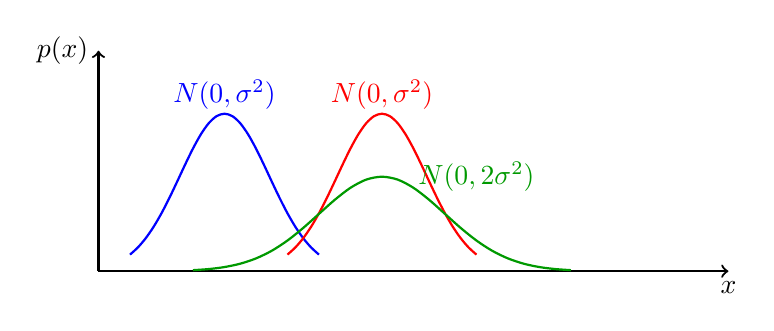
\begin{tikzpicture}[scale=0.8]
    % Axes
    \draw[thick, ->] (0,0) -- (10,0) node[below] {\( x \)};
    \draw[thick, ->] (0,0) -- (0,3.5) node[left] {\( p(x) \)};
    
    % Gaussian 1
    \draw[domain=0.5:3.5,smooth,variable=\x,blue,thick] plot ({\x},{2.5*exp(-(\x-2)^2)});
    \node[blue] at (2,2.8) {\( N(0, \sigma^2) \)};
    
    % Gaussian 2
    \draw[domain=3:6,smooth,variable=\x,red,thick] plot ({\x},{2.5*exp(-(\x-4.5)^2)});
    \node[red] at (4.5,2.8) {\( N(0, \sigma^2) \)};
    
    % Resultant Gaussian
    \draw[domain=1.5:7.5,smooth,variable=\x,green!60!black,thick] plot ({\x},{1.5*exp(-(\x-4.5)^2/2)});
    \node[green!60!black] at (6,1.5) {\( N(0, 2\sigma^2) \)};
\end{tikzpicture}
\end{center}

\subsection*{Solution 3}

We aim to explain why the probability distribution \( P(x) \) for the sum of two random variables is the convolution of their individual probability distributions. 

\subsubsection*{Step 1: Definition of Convolution}
The convolution of two probability distributions \( p_1(x) \) and \( p_2(x) \) is defined as:
\[
P(x) = (p_1 * p_2)(x) = \int_{-\infty}^\infty p_1(t) p_2(x - t) \, dt.
\]
This operation calculates the probability \( P(x) \) of obtaining the value \( x \) as a sum of two independent random variables with distributions \( p_1(x) \) and \( p_2(x) \).

\subsubsection*{Step 2: Explanation Using Dice Example}
Consider two six-sided dice, each having a uniform distribution over the numbers 1 to 6. The probability of rolling any specific number \( k \) on a die is:
\[
p_1(k) = \frac{1}{6}, \quad k = 1, 2, 3, 4, 5, 6.
\]

To compute the probability distribution \( P(x) \) of the sum \( x \) when rolling two dice, we consider all pairs \( (a, b) \) such that \( a + b = x \), where \( a \) is the result of the first die and \( b \) is the result of the second die:
\[
P(x) = \sum_{a} p_1(a) \cdot p_2(x - a).
\]
Since the dice are independent, this is equivalent to the convolution of \( p_1(x) \) and \( p_2(x) \).

\subsubsection*{Step 3: Computation for Two Dice}
For two dice, the possible sums \( x \) range from 2 to 12. The probabilities for each sum are:
\[
P(2) = \frac{1}{36}, \quad P(3) = \frac{2}{36}, \quad P(4) = \frac{3}{36}, \quad \dots, \quad P(12) = \frac{1}{36}.
\]
These probabilities are obtained by counting the number of pairs \( (a, b) \) that result in each sum \( x \) and multiplying by the individual probabilities \( \frac{1}{6} \).

\subsubsection*{Step 4: Visualization}
The following diagram illustrates the convolution process and the resulting probabilities for the sum of two dice:

\begin{center}
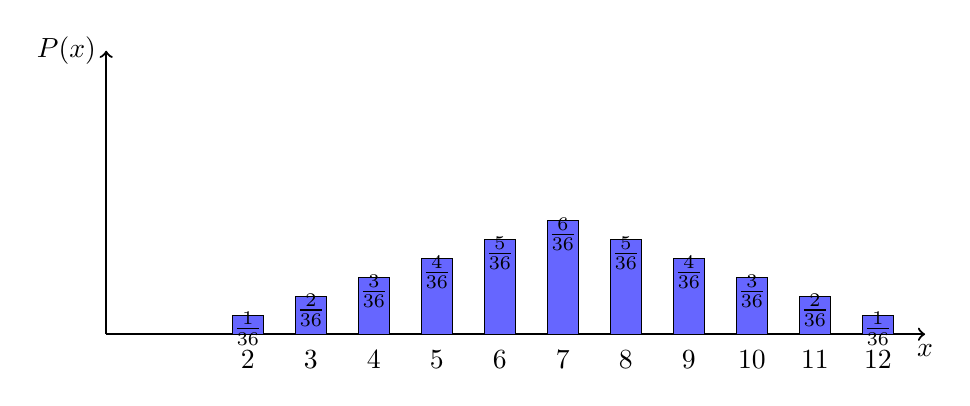
\begin{tikzpicture}[scale=0.8]
    % Axes
    \draw[thick, ->] (0,0) -- (13,0) node[below] {\( x \)};
    \draw[thick, ->] (0,0) -- (0,4.5) node[left] {\( P(x) \)};
    
    % Bars for probabilities
    \foreach \x/\y in {2/0.3, 3/0.6, 4/0.9, 5/1.2, 6/1.5, 7/1.8, 8/1.5, 9/1.2, 10/0.9, 11/0.6, 12/0.3} {
        \draw[fill=blue!60] (\x,0) rectangle (\x+0.5,\y);
    }
    
    % Labels for probabilities
    \foreach \x/\y/\p in {2/0.3/1/36, 3/0.6/2/36, 4/0.9/3/36, 5/1.2/4/36, 6/1.5/5/36, 7/1.8/6/36, 
                          8/1.5/5/36, 9/1.2/4/36, 10/0.9/3/36, 11/0.6/2/36, 12/0.3/1/36} {
        \node[below] at (\x+0.25, \y+0.2) {\(\frac{\p}{36}\)};
    }
    
    % Sum labels
    \foreach \x in {2,...,12} {
        \node[below] at (\x+0.25, -0.1) {\( \x \)};
    }
\end{tikzpicture}
\end{center}

\subsubsection*{Final Result}
The probability distribution \( P(x) \) for the sum of two random variables is their convolution:
\[
P(x) = \sum_{a} p_1(a) \cdot p_2(x - a),
\]
and for the specific case of rolling two dice, the resulting probabilities for sums \( x = 2, \dots, 12 \) are:
\[
P(x) = \left( \frac{1}{36}, \frac{2}{36}, \frac{3}{36}, \frac{4}{36}, \frac{5}{36}, \frac{6}{36}, \frac{5}{36}, \frac{4}{36}, \frac{3}{36}, \frac{2}{36}, \frac{1}{36} \right).
\]


\subsection*{Solution 4}

We aim to prove the following identity for random samples \( 0 < x_1 < x_2 < \cdots < x_n \) with probabilities \( p_1, p_2, \dots, p_n \):
\[
\textbf{mean} = E[x] = \sum_{i=1}^{n} p_i x_i = \int_{t=0}^\infty (\textbf{Probability that } x > t) \, dt.
\]

\subsubsection*{Step 1: Expected Value as a Weighted Sum}
By definition, the expected value \( E[x] \) is calculated as:
\[
E[x] = \sum_{i=1}^n p_i x_i,
\]
where \( p_i \) represents the probability associated with \( x_i \), and the terms \( x_1, x_2, \dots, x_n \) are ordered such that \( 0 < x_1 < x_2 < \cdots < x_n \).

\subsubsection*{Step 2: Probability that \( x > t \)}
The probability that \( x > t \) can be expressed as:
\[
\textbf{Probability that } x > t = 
\begin{cases} 
1, & \text{if } t < x_1, \\
1 - p_1, & \text{if } x_1 \leq t < x_2, \\
1 - p_1 - p_2, & \text{if } x_2 \leq t < x_3, \\
\vdots \\
0, & \text{if } t \geq x_n.
\end{cases}
\]

\subsubsection*{Step 3: Integration Approach}
The expected value \( E[x] \) can also be expressed as:
\[
E[x] = \int_{t=0}^\infty (\textbf{Probability that } x > t) \, dt.
\]
Substituting the piecewise definition of the probability, the integral can be broken into segments:
\[
E[x] = \int_{t=0}^{x_1} 1 \, dt 
+ \int_{t=x_1}^{x_2} (1 - p_1) \, dt 
+ \int_{t=x_2}^{x_3} (1 - p_1 - p_2) \, dt 
+ \cdots 
+ \int_{t=x_{n-1}}^{x_n} p_n \, dt.
\]

\subsubsection*{Step 4: Simplifying the Integral}
Each segment \( \int_{t=x_{i-1}}^{x_i} \) evaluates to:
\[
\int_{t=x_{i-1}}^{x_i} (1 - p_1 - \cdots - p_{i-1}) \, dt 
= (x_i - x_{i-1})(1 - p_1 - \cdots - p_{i-1}),
\]
where \( x_0 = 0 \).

Summing these contributions gives:
\[
E[x] = x_1 + (x_2 - x_1)(1 - p_1) + (x_3 - x_2)(1 - p_1 - p_2) + \cdots + (x_n - x_{n-1})p_n.
\]

\subsubsection*{Step 5: Verification of Equality}
Rearranging the terms, it can be verified that this summation is equivalent to:
\[
E[x] = \sum_{i=1}^n p_i x_i.
\]

Thus, we have shown that:
\[
E[x] = \sum_{i=1}^n p_i x_i = \int_{t=0}^\infty (\textbf{Probability that } x > t) \, dt.
\]

\subsubsection*{Visualization of the Probability Function}
The piecewise nature of the probability function can be visualized as follows:

\begin{center}
\begin{tikzpicture}[scale=1.0]
    % Axes
    \draw[thick, ->] (0,0) -- (8,0) node[below] {\( t \)};
    \draw[thick, ->] (0,0) -- (0,4) node[left] {\( \text{Probability that } x > t \)};
    
    % Horizontal lines
    \draw[thick] (0,3.5) -- (2,3.5);
    \draw[thick] (2,3.5) -- (4,2.5);
    \draw[thick] (4,2.5) -- (6,1.5);
    \draw[thick] (6,1.5) -- (8,0);
    
    % Vertical drop lines
    \draw[dashed] (2,3.5) -- (2,0);
    \draw[dashed] (4,2.5) -- (4,0);
    \draw[dashed] (6,1.5) -- (6,0);
    
    % Labels
    \node[below] at (2,0) {\( x_1 \)};
    \node[below] at (4,0) {\( x_2 \)};
    \node[below] at (6,0) {\( x_3 \)};
    \node[left] at (0,3.5) {\( 1 \)};
    \node[left] at (0,2.5) {\( 1 - p_1 \)};
    \node[left] at (0,1.5) {\( 1 - p_1 - p_2 \)};
\end{tikzpicture}
\end{center}



\subsection*{Solution 5}

Consider the Gaussian mixture model defined as:
\[
0.4 \, \mathcal{N} \left( \begin{bmatrix} 10 \\ 2 \end{bmatrix}, \begin{bmatrix} 1 & 0 \\ 0 & 1 \end{bmatrix} \right) + 0.6 \, \mathcal{N} \left( \begin{bmatrix} 0 \\ 0 \end{bmatrix}, \begin{bmatrix} 8.4 & 2.0 \\ 2.0 & 1.7 \end{bmatrix} \right).
\]

\subsubsection*{a. Marginal Distributions for Each Dimension}

For a multivariate normal distribution, the marginal distribution of each dimension is also normal, with parameters derived from the corresponding elements of the mean vector and covariance matrix.

**Component 1:**
\[
\mathcal{N} \left( \begin{bmatrix} 10 \\ 2 \end{bmatrix}, \begin{bmatrix} 1 & 0 \\ 0 & 1 \end{bmatrix} \right)
\]
- Marginal distribution for \( x_1 \): \( \mathcal{N}(10, 1) \)
- Marginal distribution for \( x_2 \): \( \mathcal{N}(2, 1) \)

**Component 2:**
\[
\mathcal{N} \left( \begin{bmatrix} 0 \\ 0 \end{bmatrix}, \begin{bmatrix} 8.4 & 2.0 \\ 2.0 & 1.7 \end{bmatrix} \right)
\]
- Marginal distribution for \( x_1 \): \( \mathcal{N}(0, 8.4) \)
- Marginal distribution for \( x_2 \): \( \mathcal{N}(0, 1.7) \)

The overall marginal distributions are weighted sums of the individual component marginals.

**Marginal Distribution for \( x_1 \):**
\[
0.4 \, \mathcal{N}(10, 1) + 0.6 \, \mathcal{N}(0, 8.4)
\]

**Marginal Distribution for \( x_2 \):**
\[
0.4 \, \mathcal{N}(2, 1) + 0.6 \, \mathcal{N}(0, 1.7)
\]

\subsubsection*{b. Mean, Mode, and Median for Each Marginal Distribution}

**Marginal Distribution for \( x_1 \):**

- **Mean:**
  \[
  E[x_1] = 0.4 \times 10 + 0.6 \times 0 = 4
  \]

- **Variance:**
  \[
  \text{Var}(x_1) = 0.4 \times (1 + (10 - 4)^2) + 0.6 \times (8.4 + (0 - 4)^2) = 25.04
  \]
  - **Standard Deviation:**
    \[
    \sigma_{x_1} = \sqrt{25.04} \approx 5.004
    \]

- **Median:**
  For a Gaussian mixture, the median does not have a closed-form solution and typically requires numerical methods for estimation.

- **Mode:**
  The mode of a Gaussian mixture is not straightforward to compute analytically and usually requires numerical optimization techniques.

**Marginal Distribution for \( x_2 \):**

- **Mean:**
  \[
  E[x_2] = 0.4 \times 2 + 0.6 \times 0 = 0.8
  \]

- **Variance:**
  \[
  \text{Var}(x_2) = 0.4 \times (1 + (2 - 0.8)^2) + 0.6 \times (1.7 + (0 - 0.8)^2) = 2.008
  \]
  - **Standard Deviation:**
    \[
    \sigma_{x_2} = \sqrt{2.008} \approx 1.417
    \]

- **Median:**
  As with \( x_1 \), the median requires numerical estimation.

- **Mode:**
  Determining the mode necessitates numerical optimization.

\subsubsection*{c. Mean and Mode for the Two-Dimensional Distribution}

- **Mean Vector:**
  \[
  E[\mathbf{x}] = 0.4 \times \begin{bmatrix} 10 \\ 2 \end{bmatrix} + 0.6 \times \begin{bmatrix} 0 \\ 0 \end{bmatrix} = \begin{bmatrix} 4 \\ 0.8 \end{bmatrix}
  \]

- **Mode:**
  The mode of a Gaussian mixture in multiple dimensions is complex to determine analytically and typically requires numerical optimization methods.




\subsection*{Solution 6}

To model the stochastic behavior of your compiler's success (\( x = 1 \)) or failure (\( x = 0 \)), we assume a Bernoulli distribution with parameter \( \mu \), representing the probability of success:

\[
p(x \mid \mu) = \mu^x (1 - \mu)^{1 - x}, \quad x \in \{0, 1\}
\]

**Conjugate Prior:**

The conjugate prior for the Bernoulli distribution is the Beta distribution, parameterized by \( \alpha \) and \( \beta \):

\[
p(\mu) = \frac{\mu^{\alpha - 1} (1 - \mu)^{\beta - 1}}{B(\alpha, \beta)}
\]

where \( B(\alpha, \beta) \) is the Beta function, serving as a normalization constant.

**Posterior Distribution:**

Given a set of \( N \) independent observations \( \{x_1, x_2, \ldots, x_N\} \), the likelihood function is:

\[
p(\{x_i\} \mid \mu) = \prod_{i=1}^N \mu^{x_i} (1 - \mu)^{1 - x_i}
\]

Combining the prior and the likelihood, the unnormalized posterior is:

\[
p(\mu \mid \{x_i\}) \propto p(\{x_i\} \mid \mu) \times p(\mu)
\]

Substituting the expressions for the likelihood and the prior:

\[
p(\mu \mid \{x_i\}) \propto \left( \prod_{i=1}^N \mu^{x_i} (1 - \mu)^{1 - x_i} \right) \times \mu^{\alpha - 1} (1 - \mu)^{\beta - 1}
\]

Simplifying the exponents by defining \( S = \sum_{i=1}^N x_i \) (the total number of successes) and \( F = N - S \) (the total number of failures):

\[
p(\mu \mid \{x_i\}) \propto \mu^{S + \alpha - 1} (1 - \mu)^{F + \beta - 1}
\]

This is the kernel of a Beta distribution with updated parameters:

\[
\mu \mid \{x_i\} \sim \text{Beta}(S + \alpha, F + \beta)
\]

**Interpretation:**

The posterior distribution \( p(\mu \mid \{x_i\}) \) is a Beta distribution with parameters:

\[
\alpha' = S + \alpha = \sum_{i=1}^N x_i + \alpha
\]
\[
\beta' = F + \beta = N - \sum_{i=1}^N x_i + \beta
\]

These updated parameters combine the prior information (\( \alpha \) and \( \beta \)) with the observed data (\( S \) successes and \( F \) failures), providing a new estimate for the probability of success \( \mu \).



\subsection*{Solution 7}

To determine the probability that the mango was picked from Bag 2, we apply Bayes' theorem. Let:

\begin{itemize}
    \item \( B_1 \): Event that the fruit is picked from Bag 1.
    \item \( B_2 \): Event that the fruit is picked from Bag 2.
    \item \( M \): Event that the fruit picked is a mango.
\end{itemize}

We aim to find \( P(B_2 \mid M) \), the probability that the fruit was picked from Bag 2 given that it is a mango.

**Bayes' Theorem:**

\[
P(B_2 \mid M) = \frac{P(M \mid B_2) \cdot P(B_2)}{P(M)}
\]

**Calculating the Components:**

1. **Prior Probabilities:**

   - \( P(B_1) \): Probability of picking from Bag 1, which occurs if the coin shows heads.

     \[
     P(B_1) = 0.6
     \]

   - \( P(B_2) \): Probability of picking from Bag 2, which occurs if the coin shows tails.

     \[
     P(B_2) = 0.4
     \]

2. **Likelihoods:**

   - \( P(M \mid B_1) \): Probability of picking a mango from Bag 1. Bag 1 contains 4 mangoes and 2 apples, totaling 6 fruits.

     \[
     P(M \mid B_1) = \frac{4}{6} = \frac{2}{3}
     \]

   - \( P(M \mid B_2) \): Probability of picking a mango from Bag 2. Bag 2 contains 4 mangoes and 4 apples, totaling 8 fruits.

     \[
     P(M \mid B_2) = \frac{4}{8} = \frac{1}{2}
     \]

3. **Total Probability of Picking a Mango, \( P(M) \):**

   Using the law of total probability:

   \[
   P(M) = P(M \mid B_1) \cdot P(B_1) + P(M \mid B_2) \cdot P(B_2)
   \]

   Substituting the known values:

   \[
   P(M) = \left( \frac{2}{3} \times 0.6 \right) + \left( \frac{1}{2} \times 0.4 \right)
   \]

   Calculating each term:

   \[
   \frac{2}{3} \times 0.6 = \frac{2 \times 0.6}{3} = \frac{1.2}{3} = 0.4
   \]

   \[
   \frac{1}{2} \times 0.4 = \frac{0.4}{2} = 0.2
   \]

   Adding these:

   \[
   P(M) = 0.4 + 0.2 = 0.6
   \]

**Applying Bayes' Theorem:**

\[
P(B_2 \mid M) = \frac{P(M \mid B_2) \cdot P(B_2)}{P(M)} = \frac{\left( \frac{1}{2} \right) \times 0.4}{0.6}
\]

Calculating the numerator:

\[
\frac{1}{2} \times 0.4 = \frac{0.4}{2} = 0.2
\]

Thus:

\[
P(B_2 \mid M) = \frac{0.2}{0.6} = \frac{1}{3} \approx 0.333
\]

**Conclusion:**

The probability that the mango was picked from Bag 2 is \( \frac{1}{3} \) or approximately 33.3\%.


\subsection*{Solution 8}

Consider the time series model:

\[
\begin{aligned}
    x_{t+1} &= \mathbf{A} x_t + \omega_t, \quad \omega_t \sim \mathcal{N}(0, Q) \\
    y_t &= \mathbf{C} x_t + v_t, \quad v_t \sim \mathcal{N}(0, R)
\end{aligned}
\]

where \( \omega_t \) and \( v_t \) are independent Gaussian noise variables. Additionally, assume that the initial state distribution is \( p(x_0) = \mathcal{N}(\mu_0, \Sigma_0) \).

**(a) Form of \( p(x_0, x_1, \dots, x_T) \):**

The joint distribution \( p(x_0, x_1, \dots, x_T) \) represents the probability of a specific sequence of states from time \( t = 0 \) to \( t = T \). Given the model's structure, this joint distribution is a multivariate Gaussian distribution. This is because:

- The initial state \( x_0 \) is Gaussian: \( x_0 \sim \mathcal{N}(\mu_0, \Sigma_0) \).

- Each subsequent state \( x_{t+1} \) is a linear transformation of \( x_t \) plus Gaussian noise \( \omega_t \). Since linear transformations and sums of Gaussian variables remain Gaussian, \( x_{t+1} \) is Gaussian if \( x_t \) is Gaussian.

By induction, all states \( x_t \) are Gaussian, and their joint distribution is a multivariate Gaussian. The mean vector and covariance matrix of this distribution can be determined recursively using the system dynamics and noise covariances.

**(b) State Estimation:**

Assume that the posterior distribution of the state at time \( t \), given all observations up to time \( T \), is Gaussian:

\[
p(x_t \mid y_1, \dots, y_T) = \mathcal{N}(\mu_t, \Sigma_t)
\]

**(b.1) Predicting \( p(x_{t+1} \mid y_1, \dots, y_T) \):**

To predict the state at time \( t+1 \) given observations up to time \( T \), we use the system's dynamics:

\[
x_{t+1} = \mathbf{A} x_t + \omega_t
\]

Taking the expectation and covariance:

\[
\begin{aligned}
    \mathbb{E}[x_{t+1} \mid y_1, \dots, y_T] &= \mathbf{A} \mathbb{E}[x_t \mid y_1, \dots, y_T] = \mathbf{A} \mu_t \\
    \text{Cov}(x_{t+1} \mid y_1, \dots, y_T) &= \mathbf{A} \Sigma_t \mathbf{A}^\top + Q
\end{aligned}
\]

Therefore, the predictive distribution is:

\[
p(x_{t+1} \mid y_1, \dots, y_T) = \mathcal{N}(\mathbf{A} \mu_t, \mathbf{A} \Sigma_t \mathbf{A}^\top + Q)
\]

**(b.2) Predicting \( y_{t+1} \) Given \( y_1, \dots, y_T \):**

The observation at time \( t+1 \) is:

\[
y_{t+1} = \mathbf{C} x_{t+1} + v_{t+1}
\]

Given \( y_1, \dots, y_T \), the predicted observation \( y_{t+1} \) has mean and covariance:

\[
\begin{aligned}
    \mathbb{E}[y_{t+1} \mid y_1, \dots, y_T] &= \mathbf{C} \mathbb{E}[x_{t+1} \mid y_1, \dots, y_T] = \mathbf{C} \mathbf{A} \mu_t \\
    \text{Cov}(y_{t+1} \mid y_1, \dots, y_T) &= \mathbf{C} \, \text{Cov}(x_{t+1} \mid y_1, \dots, y_T) \, \mathbf{C}^\top + R \\
    &= \mathbf{C} (\mathbf{A} \Sigma_t \mathbf{A}^\top + Q) \mathbf{C}^\top + R
\end{aligned}
\]

Thus, the predictive distribution for \( y_{t+1} \) is:

\[
p(y_{t+1} \mid y_1, \dots, y_T) = \mathcal{N}(\mathbf{C} \mathbf{A} \mu_t, \mathbf{C} (\mathbf{A} \Sigma_t \mathbf{A}^\top + Q) \mathbf{C}^\top + R)
\]

**(b.3) Updating \( p(x_{t+1} \mid y_1, \dots, y_{t+1}) \) After Observing \( y_{t+1} = \hat{y} \):**

Upon observing \( y_{t+1} = \hat{y} \), we update our estimate of \( x_{t+1} \) using the Kalman filter update equations:

- **Kalman Gain:**

  \[
  K_{t+1} = \Sigma_{t+1 \mid t} \mathbf{C}^\top (\mathbf{C} \Sigma_{t+1 \mid t} \mathbf{C}^\top + R)^{-1}
  \]

  where \( \Sigma_{t+1 \mid t} = \mathbf{A} \Sigma_t \mathbf{A}^\top + Q \) is the prior covariance of \( x_{t+1} \).

- **Updated Mean:**

  \[
  \mu_{t+1} = \mu_{t+1 \mid t} + K_{t+1} (\hat{y} - \mathbf{C} \mu_{t+1 \mid t})
  \]

  with \( \mu_{t+1 \mid t} = \mathbf{A} \mu_t \) being the prior mean of \( x_{t+1} \).

- **Updated Covariance:**

  \[
  \Sigma_{t+1} = (\mathbf{I} - K_{t+1} \mathbf{C}) \Sigma_{t+1 \mid t}
  \]

Therefore, the updated distribution is:

\[
p(x_{t+1} \mid y_1, \dots, y_{t+1}) = \mathcal{N
::contentReference[oaicite:0]{index=0}




\section*{Solution 9}
\textbf{Manipulation of Gaussian Random Variables}

Consider a Gaussian random variable \( \mathbf{x} \sim \mathcal{N}(\bm{\mu}_x, \bm{\Sigma}_x) \), where \( \mathbf{x} \in \mathbb{R}^D \). Furthermore, we have
\[
\mathbf{y} = A\mathbf{x} + \mathbf{b} + \bm{\omega},
\]
where \( \mathbf{y} \in \mathbb{R}^E \), \( A \in \mathbb{R}^{E \times D} \), \( \mathbf{b} \in \mathbb{R}^E \), and \( \bm{\omega} \sim \mathcal{N}(\mathbf{0}, Q) \) is independent Gaussian noise. ``Independent'' implies that \( \mathbf{x} \) and \( \bm{\omega} \) are independent random variables and that \( Q \) is diagonal.

\subsection*{a. Likelihood \( p(\mathbf{y} \mid \mathbf{x}) \)}

Given \( \mathbf{x} \), the distribution of \( \mathbf{y} \) is determined by the linear transformation and the additive Gaussian noise \( \bm{\omega} \). Therefore, the likelihood \( p(\mathbf{y} \mid \mathbf{x}) \) is Gaussian:
\[
p(\mathbf{y} \mid \mathbf{x}) = \mathcal{N}(\mathbf{y} \mid A\mathbf{x} + \mathbf{b}, Q).
\]

\subsection*{b. Distribution \( p(\mathbf{y}) \)}

To find the distribution of \( \mathbf{y} \), we note that it is a linear transformation of \( \mathbf{x} \) with added Gaussian noise \( \bm{\omega} \). Since both \( \mathbf{x} \) and \( \bm{\omega} \) are Gaussian and independent, \( \mathbf{y} \) is also Gaussian. The mean and covariance of \( \mathbf{y} \) are given by:
\[
\bm{\mu}_y = A\bm{\mu}_x + \mathbf{b},
\]
\[
\bm{\Sigma}_y = A\bm{\Sigma}_x A^\top + Q.
\]
This follows from the properties of linear transformations of Gaussian random variables \cite{turn0search0}.

\subsection*{c. Measurement Mapping}

Given the transformation
\[
\mathbf{z} = C\mathbf{y} + \mathbf{v},
\]
where \( \mathbf{z} \in \mathbb{R}^F \), \( C \in \mathbb{R}^{F \times E} \), and \( \mathbf{v} \sim \mathcal{N}(\mathbf{0}, R) \) is independent Gaussian noise:

\subsubsection*{i. Likelihood \( p(\mathbf{z} \mid \mathbf{y}) \)}

The likelihood \( p(\mathbf{z} \mid \mathbf{y}) \) is Gaussian:
\[
p(\mathbf{z} \mid \mathbf{y}) = \mathcal{N}(\mathbf{z} \mid C\mathbf{y}, R).
\]

\subsubsection*{ii. Distribution \( p(\mathbf{z}) \)}

Since \( \mathbf{z} \) is a linear transformation of \( \mathbf{y} \) with added Gaussian noise \( \mathbf{v} \), and \( \mathbf{y} \) is Gaussian, \( \mathbf{z} \) is also Gaussian. The mean and covariance of \( \mathbf{z} \) are:
\[
\bm{\mu}_z = C\bm{\mu}_y = C(A\bm{\mu}_x + \mathbf{b}),
\]
\[
\bm{\Sigma}_z = C\bm{\Sigma}_y C^\top + R = C(A\bm{\Sigma}_x A^\top + Q)C^\top + R.
\]

\subsection*{d. Posterior Distribution \( p(\mathbf{x} \mid \hat{\mathbf{y}}) \)}

Given a measurement \( \hat{\mathbf{y}} \), we seek the posterior distribution \( p(\mathbf{x} \mid \hat{\mathbf{y}}) \). Since \( \mathbf{x} \) and \( \mathbf{y} \) are jointly Gaussian, the posterior distribution is also Gaussian. The joint distribution \( p(\mathbf{x}, \mathbf{y}) \) is:
\[
\begin{bmatrix}
\mathbf{x} \\
\mathbf{y}
\end{bmatrix}
\sim \mathcal{N}\left(
\begin{bmatrix}
\bm{\mu}_x \\
\bm{\mu}_y
\end{bmatrix},
\begin{bmatrix}
\bm{\Sigma}_x & \bm{\Sigma}_{xy} \\
\bm{\Sigma}_{yx} & \bm{\Sigma}_y
\end{bmatrix}
\right),
\]
where \( \bm{\Sigma}_{xy} = \bm{\Sigma}_x A^\top \) and \( \bm{\Sigma}_{yx} = A\bm{\Sigma}_x \).

The conditional distribution \( p(\mathbf{x} \mid \hat{\mathbf{y}}) \) is Gaussian with mean and covariance:
\[
\bm{\mu}_{\mathbf{x} \mid \hat{\mathbf{y}}} = \bm{\mu}_x + \bm{\Sigma}_{xy} \bm{\Sigma}_y^{-1} (\hat{\mathbf{y}} - \bm{\mu}_y),
\]
\[
\bm{\Sigma}_{\mathbf{x} \mid \hat{\mathbf{y}}} = \bm{\Sigma}_x - \bm{\Sigma}_{xy} \bm{\Sigma}_y^{-1} \bm{\Sigma}_{yx}.
\]
These results are derived from the properties of conditional distributions of jointly Gaussian random variables



\section*{Solution 10}


\subsection*{Part 1: Methodology}

We aim to compute the standardized variable:
\[
X = \frac{A_N - \frac{1}{2}}{2 \sqrt{N}}
\]
where \( A_N \) is the average of \( N \) random 0-1 samples.

\subsubsection*{Sample Mean (\( A_N \))}

\begin{itemize}
    \item Each sample is a Bernoulli random variable with parameter \( p = 0.5 \).
    \item The mean of a Bernoulli random variable is \( p \), and the variance is \( p(1 - p) \).
    \item For \( p = 0.5 \), both mean and variance are \( 0.25 \).
    \item The sample mean \( A_N \) is an unbiased estimator of \( p \).
\end{itemize}

\subsubsection*{Standardization}

\begin{itemize}
    \item The standard deviation of the sample mean \( A_N \) is \( \sqrt{\frac{p(1 - p)}{N}} = \frac{1}{2\sqrt{N}} \).
    \item Standardizing \( A_N \) involves subtracting the mean and dividing by the standard deviation:
    \[
    Z = \frac{A_N - \frac{1}{2}}{\frac{1}{2\sqrt{N}}} = 2\sqrt{N} \left( A_N - \frac{1}{2} \right)
    \]
    \item Comparing this with the given expression for \( X \), we see:
    \[
    X = \frac{A_N - \frac{1}{2}}{2 \sqrt{N}} = \frac{1}{4N} \times Z
    \]
    \item Therefore, \( X \) is a scaled version of the standard normal variable \( Z \).
\end{itemize}

\subsubsection*{Expected Value of \( X \)}

\begin{itemize}
    \item Since \( Z \) follows a standard normal distribution with mean 0, the expected value of \( X \) is also 0.
\end{itemize}

\subsubsection*{Variance of \( X \)}

\begin{itemize}
    \item The variance of \( Z \) is 1.
    \item The variance of \( X \) is:
    \[
    \text{Var}(X) = \left( \frac{1}{4N} \right)^2 \times \text{Var}(Z) = \frac{1}{16N^2}
    \]
\end{itemize}

\subsection*{Part 2: Python Code}

\begin{lstlisting}
import numpy as np

# Number of samples
N = 1_000_000

# Generate N random samples from a Bernoulli distribution with p=0.5
samples = np.random.binomial(n=1, p=0.5, size=N)

# Compute the sample mean
A_N = np.mean(samples)

# Compute the standardized variable X
X = (A_N - 0.5) / (2 * np.sqrt(N))

# Output the results
print(f"Sample Mean (A_N): {A_N}")
print(f"Standardized Variable (X): {X}")
\end{lstlisting}

\section*{Solution 11}

\subsection*{Part 1: Methodology}

\subsubsection*{1. Download and Summarize the Dataset}

\begin{itemize}
    \item The dataset contains measurements for three penguin species: Adelie, Gentoo, and Chinstrap.
    \item Features include:
    \begin{itemize}
        \item \texttt{species}: Penguin species.
        \item \texttt{island}: Island in the Palmer Archipelago.
        \item \texttt{culmen\_length\_mm}: Bill length (mm).
        \item \texttt{culmen\_depth\_mm}: Bill depth (mm).
        \item \texttt{flipper\_length\_mm}: Flipper length (mm).
        \item \texttt{body\_mass\_g}: Body mass (g).
        \item \texttt{sex}: Gender of the penguin.
    \end{itemize}
    \item The dataset may contain missing values that need to be addressed.
\end{itemize}

\subsubsection*{2. Exploratory Data Analysis (EDA)}

\begin{itemize}
    \item Visualize distributions of numerical features.
    \item Analyze relationships between features using scatter plots and pair plots.
    \item Examine differences between species.
    \item Handle missing values appropriately.
\end{itemize}

\subsubsection*{3. Identify Clusters}

\begin{itemize}
    \item Apply clustering algorithms such as K-Means to identify natural groupings.
    \item Use dimensionality reduction techniques like PCA for visualization.
    \item Evaluate clustering performance using metrics like silhouette score.
\end{itemize}

\subsubsection*{4. Predict Species of a Given Penguin}

\begin{itemize}
    \item Consider supervised learning algorithms:
    \begin{itemize}
        \item Logistic Regression
        \item Decision Trees
        \item Random Forests
        \item Support Vector Machines
        \item k-Nearest Neighbors
    \end{itemize}
    \item Evaluate models using cross-validation and metrics such as accuracy, precision, recall, and F1-score.
    \item Select the best model based on performance metrics.
\end{itemize}

\subsection*{Part 2: Python Code}

\begin{lstlisting}
# Import necessary libraries
import pandas as pd
import seaborn as sns
import matplotlib.pyplot as plt
from sklearn.cluster import KMeans
from sklearn.decomposition import PCA
from sklearn.preprocessing import StandardScaler
from sklearn.metrics import silhouette_score
from sklearn.model_selection import train_test_split
from sklearn.ensemble import RandomForestClassifier
from sklearn.metrics import classification_report, confusion_matrix

# Load the dataset
url = 'https://github.com/mwaskom/seaborn-data/raw/master/penguins.csv'
penguins = pd.read_csv(url)

# Display the first few rows of the dataset
print(penguins.head())

# Summary statistics
print(penguins.describe())

# Check for missing values
print(penguins.isnull().sum())

# Drop rows with missing values for simplicity
penguins.dropna(inplace=True)

# Exploratory Data Analysis (EDA)
# Pair plot to visualize relationships between features
sns.pairplot(penguins, hue='species')
plt.show()

# Box plots to visualize distributions
plt.figure(figsize=(12, 6))
sns.boxplot(x='species', y='culmen_length_mm', data=penguins)
plt.title('Culmen Length by Species')
plt.show()

# Clustering
# Select numerical features for clustering
features = ['culmen_length_mm', 'culmen_depth_mm', 'flipper_length_mm', 'body_mass_g']
X = penguins[features]

# Standardize the features
scaler = StandardScaler()
X_scaled = scaler.fit_transform(X)

# Apply K-Means clustering
kmeans = KMeans(n_clusters=3, random_state=42)
penguins['cluster'] = kmeans.fit_predict(X_scaled)

# Evaluate clustering performance
silhouette_avg = silhouette_score(X_scaled, penguins['cluster'])
print(f'Silhouette Score: {silhouette_avg}')

# Visualize clusters using PCA
pca = PCA(n_components=2)
principal_components = pca.fit_transform(X_scaled)
penguins['pca1'] = principal_components[:, 0]
penguins['pca2'] = principal_components[:, 1]

plt.figure(figsize=(10, 6))
sns.scatterplot(x='pca1', y='pca2', hue='cluster', data=penguins, palette='Set1')
plt.title('PCA of Penguin Clusters')
plt.show()

# Predicting Species
# Encode categorical variables
penguins['sex'] = penguins['sex'].map({'Male': 0, 'Female': 1})
penguins = pd.get_dummies(penguins, columns=['island'], drop_first=True)

# Define feature matrix and target vector
X = penguins.drop(columns=['species', 'cluster', 'pca1', 'pca2'])
y = penguins['species']

# Split the data into training and testing sets
X_train, X_test, y_train, y_test = train_test_split(X, y, test_size=0.2, random_state=42)

# Train a Random Forest Classifier
rf = RandomForestClassifier(n_estimators=100, random_state=42)
rf.fit(X_train, y_train)

# Make predictions
y_pred = rf.predict(X_test)

# Evaluate the model
print(confusion_matrix(y_test, y_pred))
print(classification_report(y_test, y_pred))
\end{lstlisting}




\section*{Dataset Collection and Analysis}

The following dataset have been used to perform the analysis:
\href{https://www.kaggle.com/datasets/ashaychoudhary/panic-attack-dataset}{Download Dataset Here}

The colab notebook containing the code is attached below for reference:
\href{https://colab.research.google.com/drive/1_Y1EvOdor7KVAh8MZmtfsyvm0QcEUzmu?usp=sharing}{Colab Notebook}

\begin{lstlisting}
from google.colab import drive

drive.mount("/content/drive")

import pandas as pd
import numpy as np
import seaborn as sns
from scipy.stats import zscore
import matplotlib.pyplot as plt

df = pd.read_csv("/content/drive/MyDrive/Course Work/Sem 4/Data Analysis and Visualization/Homework 1/panic_attack_dataset.csv")

df.head()

print("Dataset Information")
df.info()

print("Summary Statistics")
df.describe(include="all")

print("Missing Values")
df.isnull().sum()

# Dataset Cleaning

# Handling missing values i.e. filling numerical columns with means and categorical columns with mode
for col in df.select_dtypes(include=[np.number]).columns:
    df[col].fillna(df[col].mean(), inplace=True)

for col in df.select_dtypes(include=[object]).columns:
    df[col].fillna(df[col].mode()[0], inplace=True)

df.drop_duplicates(inplace=True)

df.describe(include="all")

for col in df.select_dtypes(include=[object]).columns:
    print(col, df[col].unique())

for col in df.select_dtypes(include=[object]).columns:
    df[col] = df[col].str.lower().str.strip()

for col in df.select_dtypes(include=[object]).columns:
    print(col, df[col].unique())

# Outlier detection and removal
z_scores = np.abs(zscore(df.select_dtypes(include=[np.number])))
outliers = (z_scores > 3).any(axis=1)
print(outliers.sum())

df = df[~outliers]

# Univariate Analysis
# Numerical columns
for col in df.select_dtypes(include=[np.number]).columns:
    plt.figure(figsize=(8, 5))
    sns.histplot(df[col], kde=True, bins=30)
    plt.title(f"Distribution of {col}")
    plt.show()

for col in df.select_dtypes(include=[object]).columns:
    plt.figure(figsize=(8, 5))
    sns.countplot(data=df, x=col, order=df[col].value_counts().index)
    plt.title(f"Distribution of {col}")
    plt.xticks(rotation=45)
    plt.show()

# Bivariate Analysis
numeric_df = df.select_dtypes(include=[np.number])
plt.figure(figsize=(10, 8))
sns.heatmap(numeric_df.corr(), annot=True, cmap="coolwarm", fmt=".2f")
plt.title("Correlation Matrix")
plt.show()

sns.pairplot(df.select_dtypes(include=[np.number]), diag_kind="kde")
plt.show()

numeric_df = df.select_dtypes(include=[np.number])
correlation_matrix = numeric_df.corr().unstack().sort_values(ascending=False)
correlation_matrix = correlation_matrix[correlation_matrix < 1]
print("Top Correlations: ")
print(correlation_matrix.head(10))
\end{lstlisting}


















 

 









\end{document}
